\begingroup
\renewcommand*{\arraystretch}{1.5}
\begin{table}[h!]
	\centering
	\begin{tabular}{c | c | c | c}
		\multirow{2}{*}{$ w_0 $ [$ \mu\mathrm{m} $]} & \multicolumn{3}{c}{Total absorption of laser energy [\%]} \\ \cline{2-4}
		 & const. E = $ 2.83 \cdot 10^{4} $ J & const. I = $ 10^{20} $ W/cm$^2$ & const. I = $ 10^{21} $ W/cm$^2$ \\ \hline \hline
		0.5 & 20.12 & 16.23 & 31.77 \\ \hline
		1.0 & 9.59 & 9.59 & 23.76 \\ \hline
		2.0 & 5.27 & 8.26 & 23.82 \\ \hline
		4.0 & 3.49 & 8.29 & 23.71 \\
	\end{tabular}
	\caption{A summary of the values of the total laser light absorption in plasma for several different sizes of the focal spot and different laser intensities.}
	\label{table:4}
\end{table}
\endgroup

\floatsetup[figure]{style=plain, subcapbesideposition=top}
\begin{figure}[h!]
	\centering
	\sidesubfloat[]{{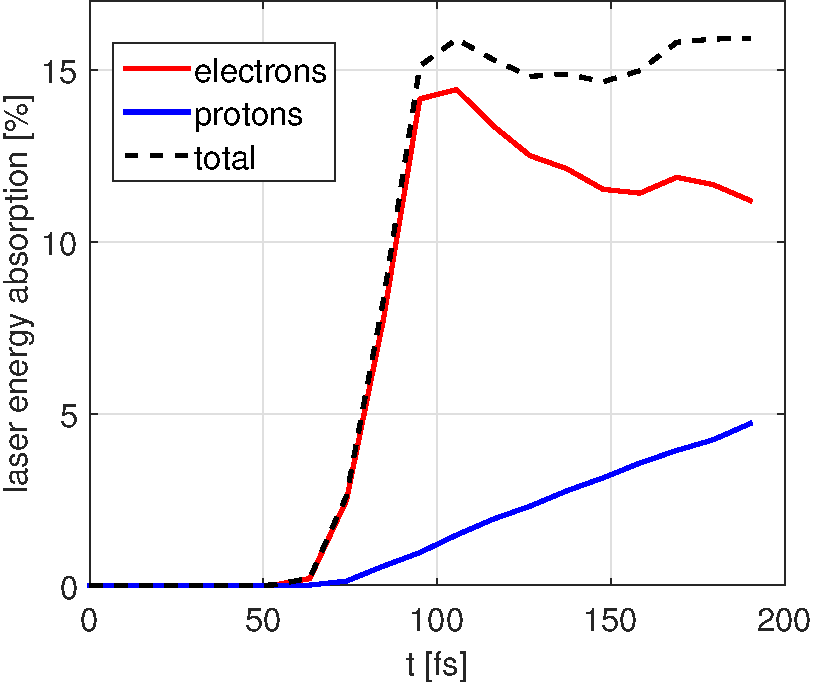
\includegraphics[width=0.45\linewidth]{./img/results/i1e20/05/absorp.pdf}}}
	\sidesubfloat[]{{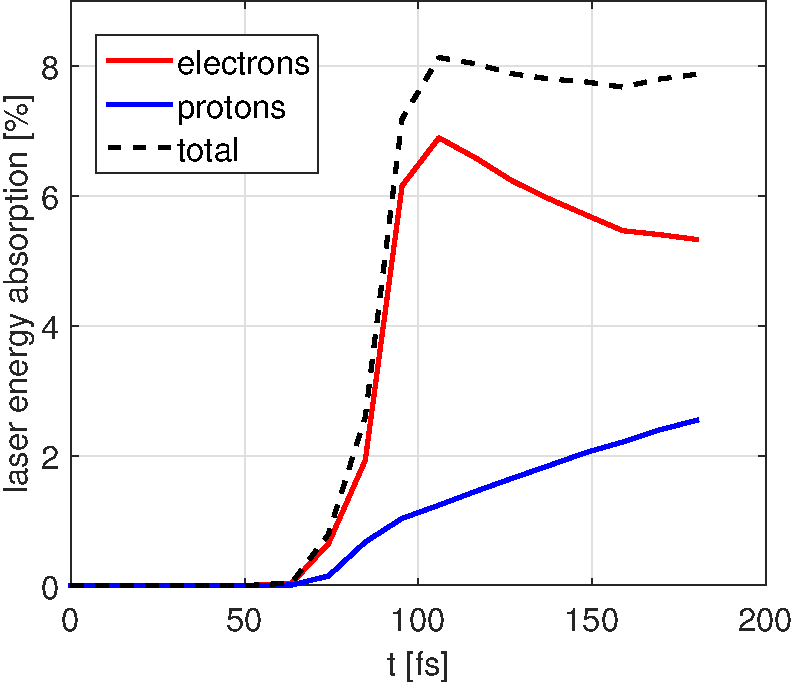
\includegraphics[width=0.45\linewidth]{./img/results/i1e20/2/absorp.pdf}}}\\
	\sidesubfloat[]{{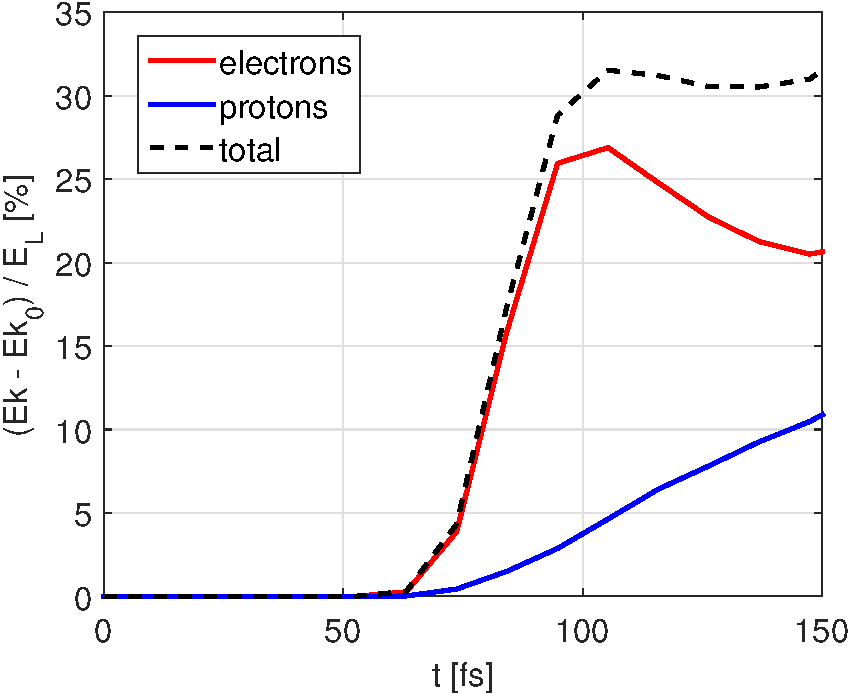
\includegraphics[width=0.45\linewidth]{./img/results/i1e21/05/absorp.pdf}}}
	\sidesubfloat[]{{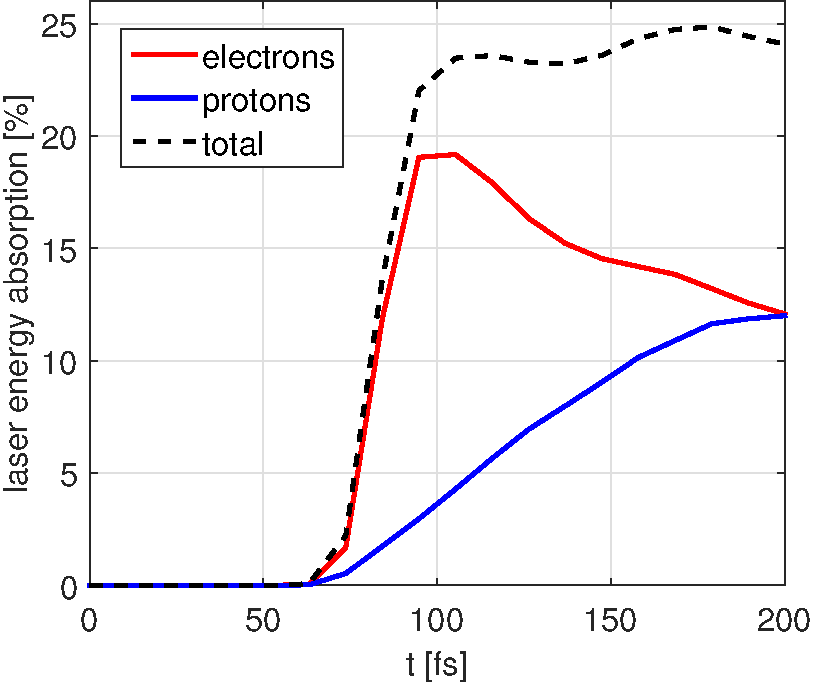
\includegraphics[width=0.45\linewidth]{./img/results/i1e21/2/absorp.pdf}}}
	\caption{Laser energy absorption in time for the case of simulations with the laser intensity I = $ 10^{20} $ W/cm$^2$ and with the beam waist \textbf{(a)} $ w_0 = 0.5 \ \mu\mathrm{m} $, \textbf{(b)} $ w_0 = 2.0 \ \mu\mathrm{m} $ and for the case of simulations with the laser intensity I = $ 10^{21} $ W/cm$^2$ and with the beam waist \textbf{(c)} $ w_0 = 0.5 \ \mu\mathrm{m} $, \textbf{(d)} $ w_0 = 2.0 \ \mu\mathrm{m} $.}
	\label{fig:10}
\end{figure}

\floatsetup[figure]{style=plain, subcapbesideposition=top}
\begin{figure}[h!]
	\centering
	\sidesubfloat[]{{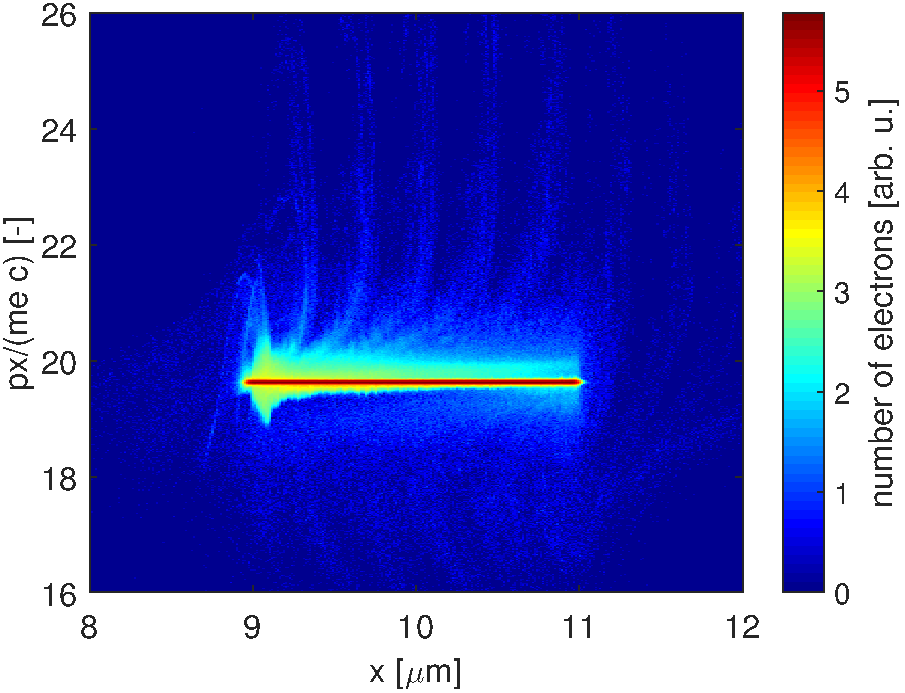
\includegraphics[width=0.45\linewidth]{./img/results/i1e20/05/x_px.pdf}}}
	\sidesubfloat[]{{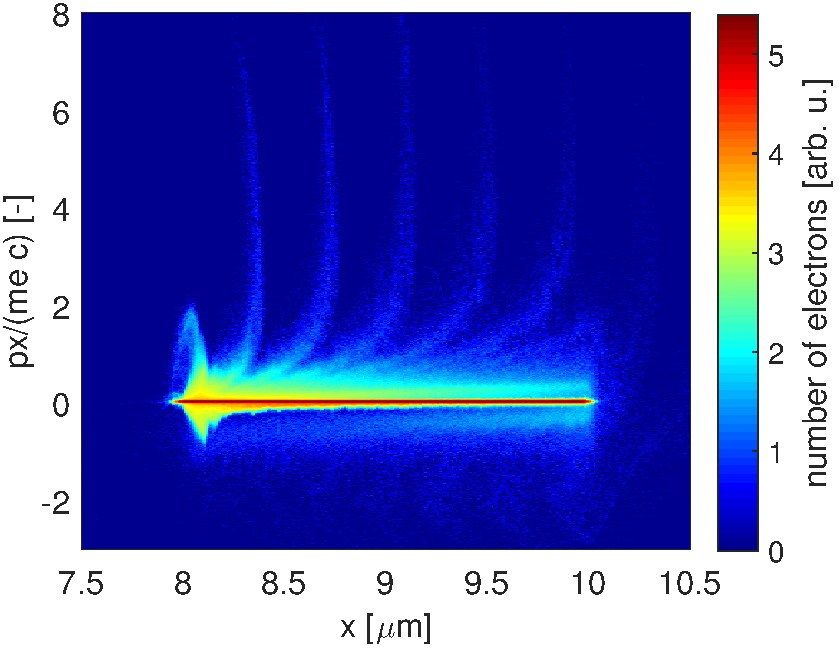
\includegraphics[width=0.45\linewidth]{./img/results/i1e20/2/x_px.pdf}}}\\
	\sidesubfloat[]{{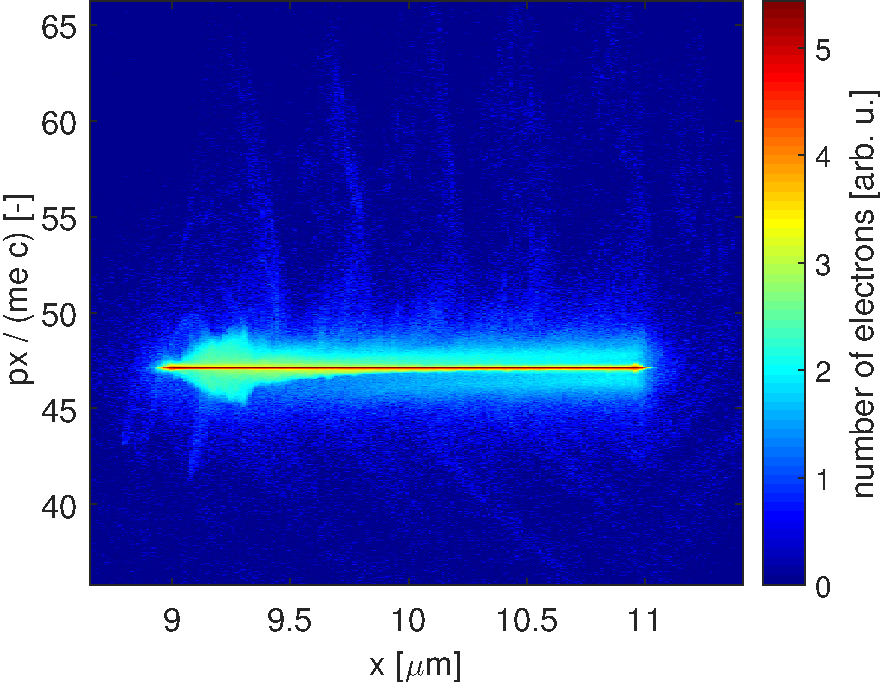
\includegraphics[width=0.45\linewidth]{./img/results/i1e21/05/x_px.pdf}}}
	\sidesubfloat[]{{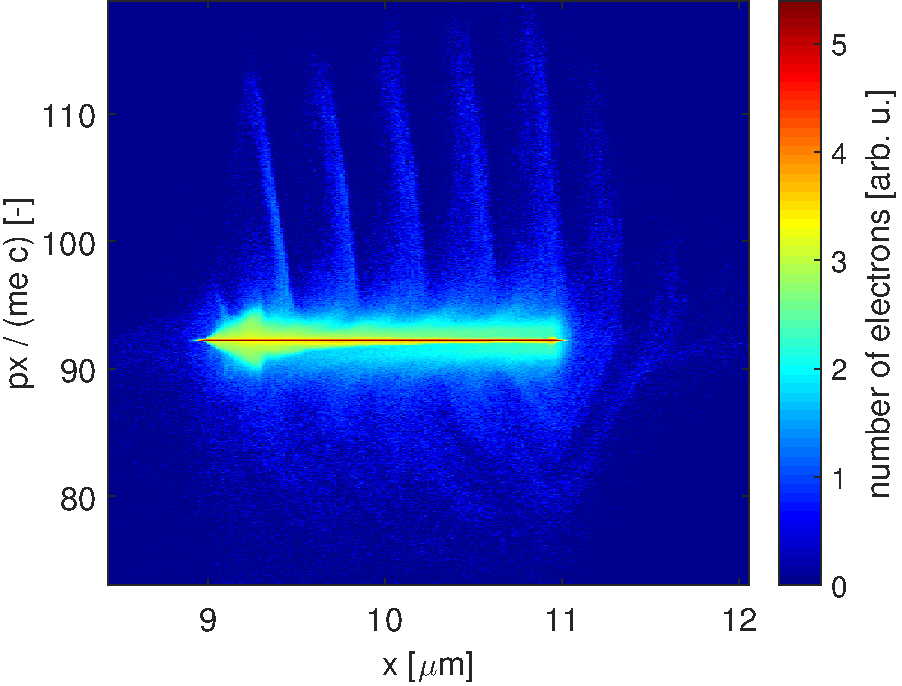
\includegraphics[width=0.45\linewidth]{./img/results/i1e21/2/x_px.pdf}}}
	\caption{Dependency of the x-component of the momentum of electrons on the x-coordinate at the time $ t = 100 \ \mathrm{fs} $ for the case of simulations with the laser intensity I = $ 10^{20} $ W/cm$^2$ and with the beam waist \textbf{(a)} $ w_0 = 0.5 \ \mu\mathrm{m} $, \textbf{(b)} $ w_0 = 2.0 \ \mu\mathrm{m} $ and for the case of simulations with the laser intensity I = $ 10^{21} $ W/cm$^2$ and with the beam waist \textbf{(c)} $ w_0 = 0.5 \ \mu\mathrm{m} $, \textbf{(d)} $ w_0 = 2.0 \ \mu\mathrm{m} $. The colorbars are in logarithmic scale.}
	\label{fig:11}
\end{figure}

\floatsetup[figure]{style=plain, subcapbesideposition=top}
\begin{figure}[h!]
	\centering
	\sidesubfloat[]{{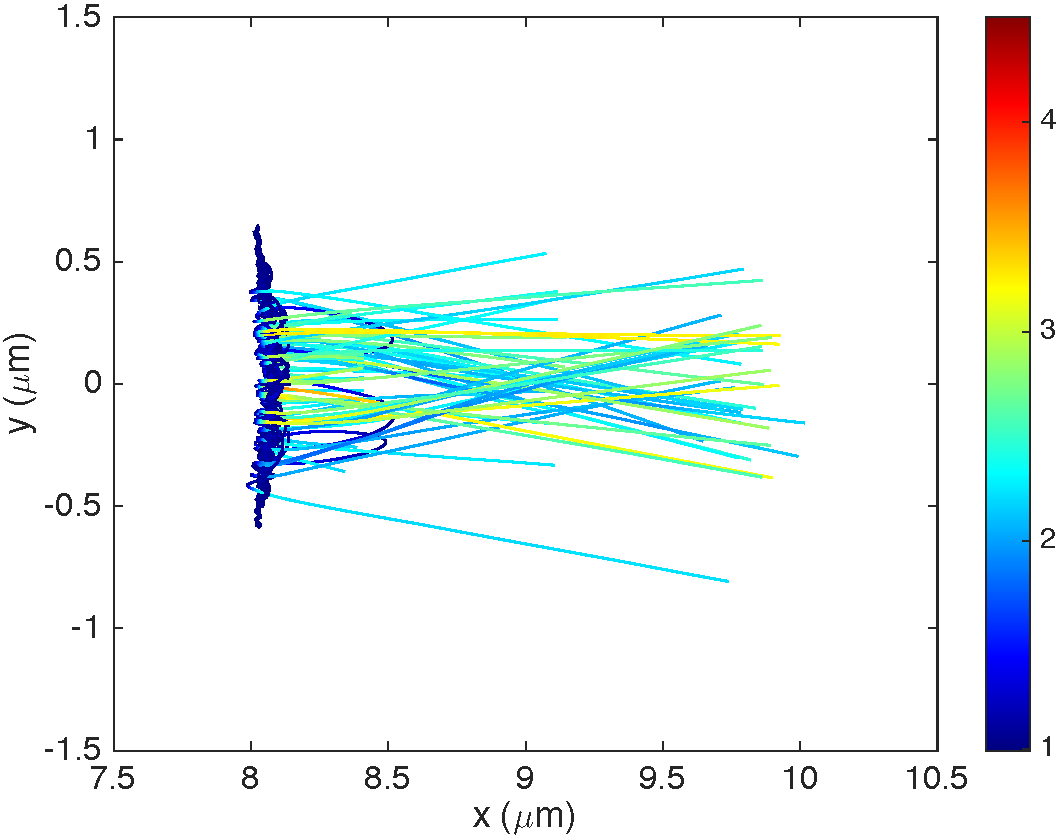
\includegraphics[width=0.4\linewidth]{./img/results/i1e20/05/traj_1.pdf}}}
	\sidesubfloat[]{{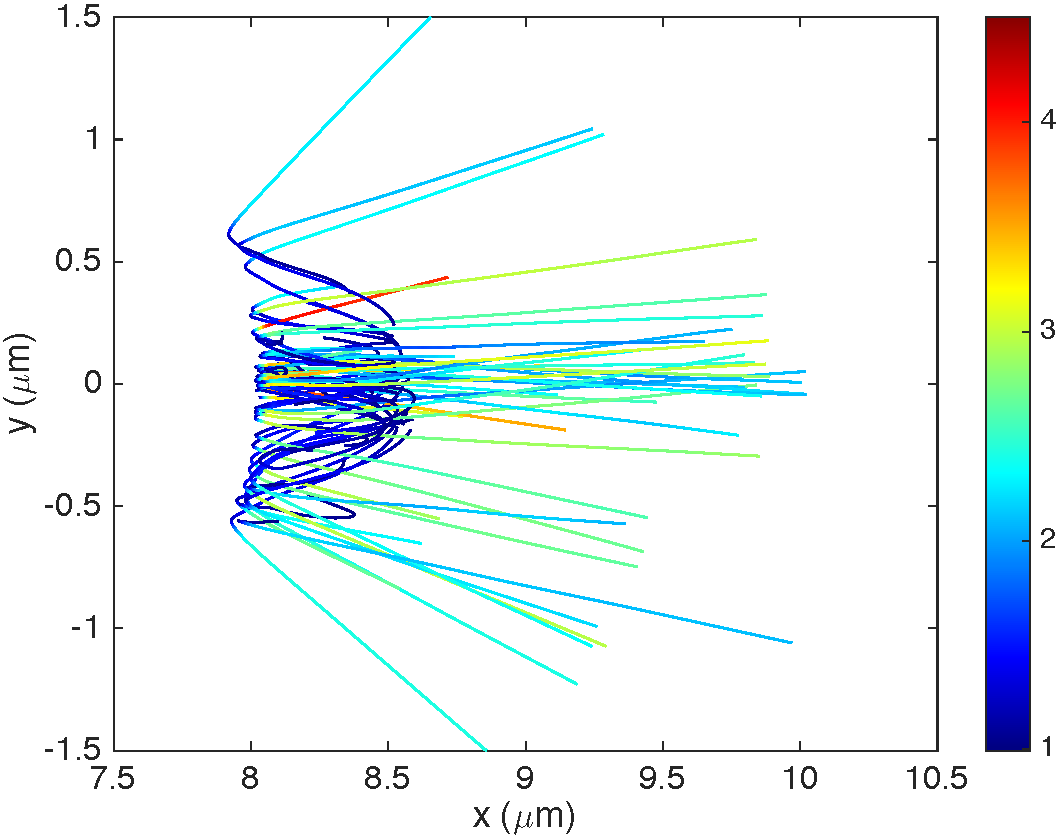
\includegraphics[width=0.4\linewidth]{./img/results/i1e20/05/traj_2.pdf}}}\\[2mm]
	\sidesubfloat[]{{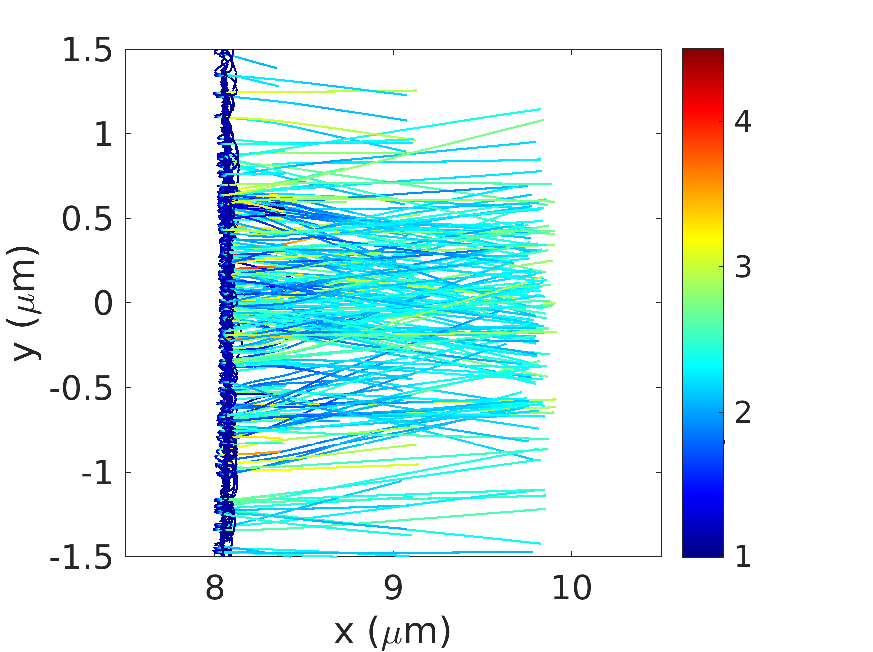
\includegraphics[width=0.4\linewidth]{./img/results/i1e20/2/traj_1.pdf}}}
	\sidesubfloat[]{{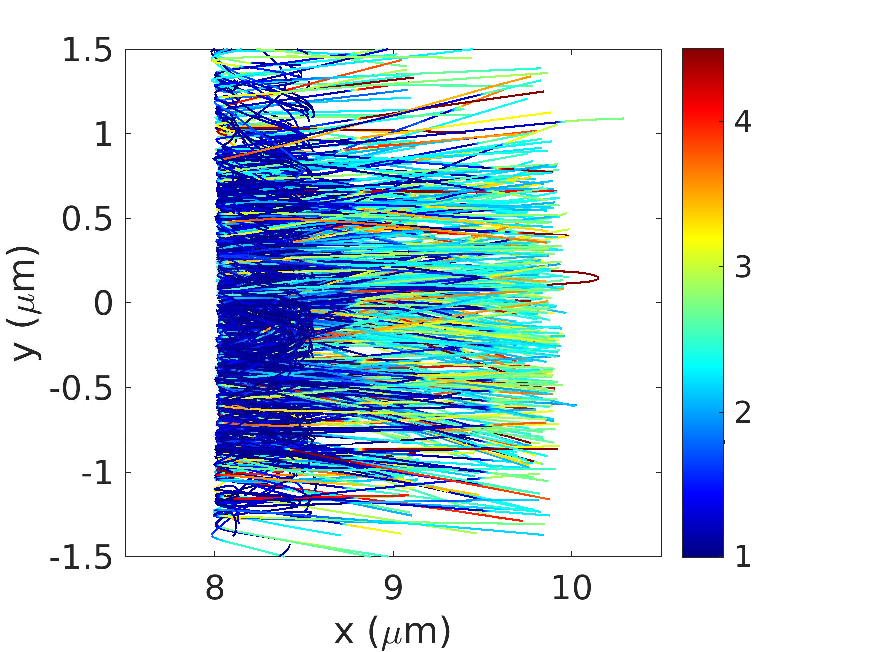
\includegraphics[width=0.4\linewidth]{./img/results/i1e20/2/traj_2.pdf}}}
	\caption{Two types of trajectories of randomly chosen electron samples for the case of simulations with the laser intensity I = $ 10^{20} $ W/cm$^2$ and with the beam waist \textbf{(a), (b)} $ w_0 = 0.5 \ \mu\mathrm{m} $ and \textbf{(c), (d)} $ w_0 = 2.0 \ \mu\mathrm{m} $. The trajectories are colored according to the Lorentz gamma factor of corresponding particles.}
	\label{fig:19}
\end{figure}

\floatsetup[figure]{style=plain, subcapbesideposition=top}
\begin{figure}[h!]
	\centering
	\sidesubfloat[]{{\includegraphics[width=0.45\linewidth]{./img/results/i1e20/05/fpx.pdf}}}
	\sidesubfloat[]{{\includegraphics[width=0.45\linewidth]{./img/results/i1e20/05/fpy.pdf}}}\\
	\sidesubfloat[]{{\includegraphics[width=0.45\linewidth]{./img/results/i1e20/2/fpx.pdf}}}
	\sidesubfloat[]{{\includegraphics[width=0.45\linewidth]{./img/results/i1e20/2/fpy.pdf}}}
	\caption{The x-component of ponderomotive force $ F_{p, x} $ \textbf{(a)} and the y-component of ponderomotive force $ F_{p, y} $ \textbf{(b)} for the case of the laser beam with intensity I = $ 10^{20} $ W/cm$^2$ and the beam waist $ w_0 = 0.5 \ \mu\mathrm{m} $ propagating in vacuum. The x-component of ponderomotive force $ F_{p, x} $ \textbf{(c)} and the y-component of ponderomotive force $ F_{p, y} $ \textbf{(d)} for the case of the laser beam with intensity I = $ 10^{20} $ W/cm$^2$ and the beam waist $ w_0 = 2.0 \ \mu\mathrm{m} $ propagating in vacuum. (max: \textbf{(a)} 5.1312e-06 \textbf{(b)} 1.5913e-06 ... pomer: x:y = 3.2:1 \textbf{(c)} 5.9528e-06 \textbf{(d)} 4.6193e-07 ... pomer: x:y = 12.8:1)}
	\label{fig:21}
\end{figure}

\floatsetup[figure]{style=plain, subcapbesideposition=top}
\begin{figure}[h!]
	\centering
	\sidesubfloat[]{{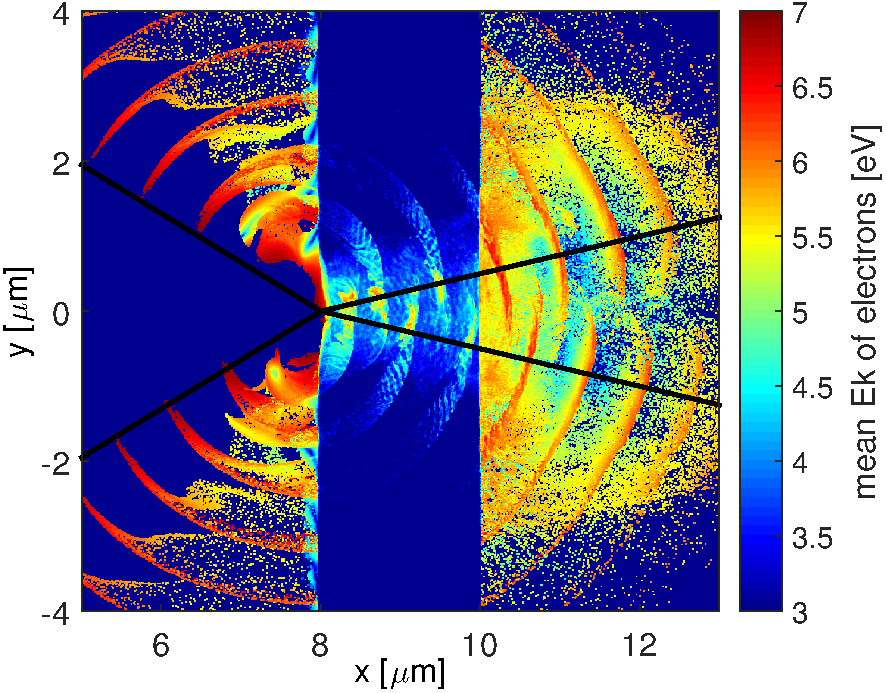
\includegraphics[width=0.45\linewidth]{./img/results/i1e21/05/ekbar_2.pdf}}}
	\sidesubfloat[]{{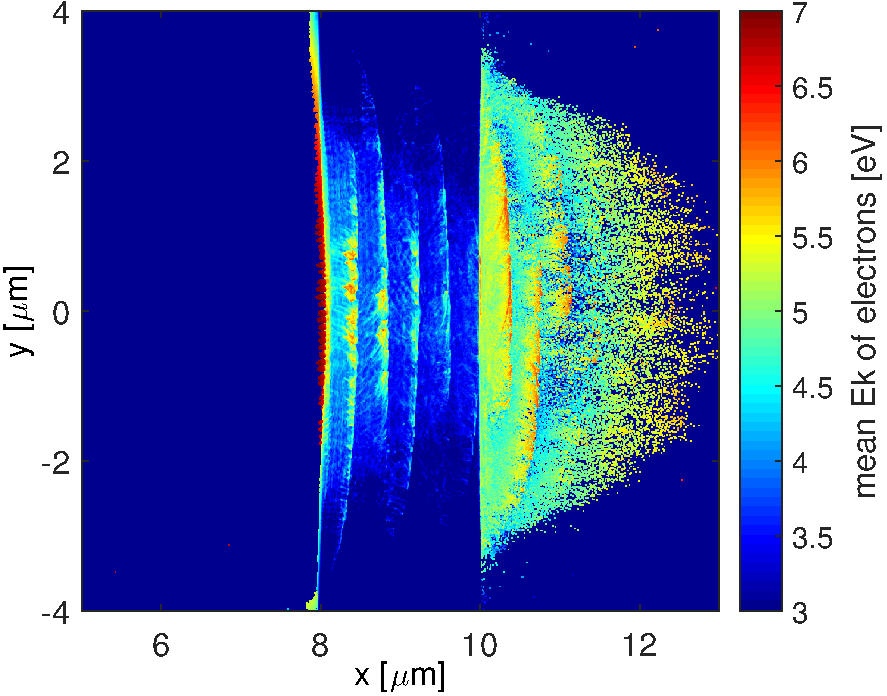
\includegraphics[width=0.45\linewidth]{./img/results/i1e21/2/ekbar_2.pdf}}}\\[2mm]
	\caption{Mean kinetic energy of electrons at the time $ t = 80 \ \mathrm{fs} $ for the case of simulations with the laser intensity I = $ 10^{21} $ W/cm$^2$ and with the beam waist \textbf{(a)} $ w_0 = 0.5 \ \mu\mathrm{m} $, \textbf{(b)} $ w_0 = 2.0 \ \mu\mathrm{m} $. The colorbars are in logarithmic scale.}
	\label{fig:17}
\end{figure}

\floatsetup[figure]{style=plain, subcapbesideposition=top}
\begin{figure}[h!]
	\centering
	\sidesubfloat[]{{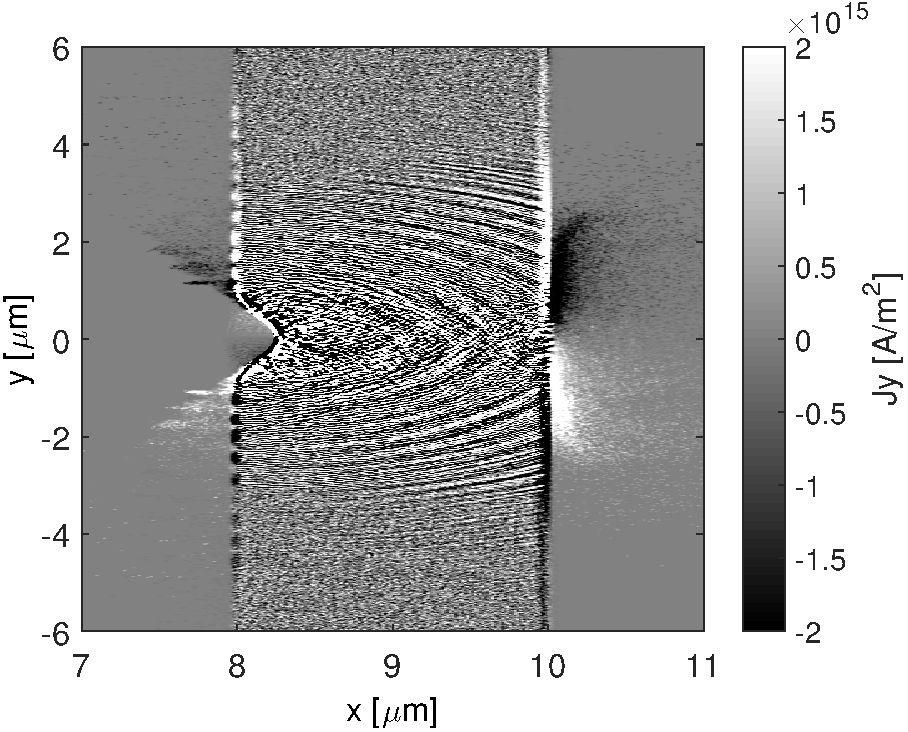
\includegraphics[width=0.45\linewidth]{./img/results/i1e21/05/jy.pdf}}}
	\sidesubfloat[]{{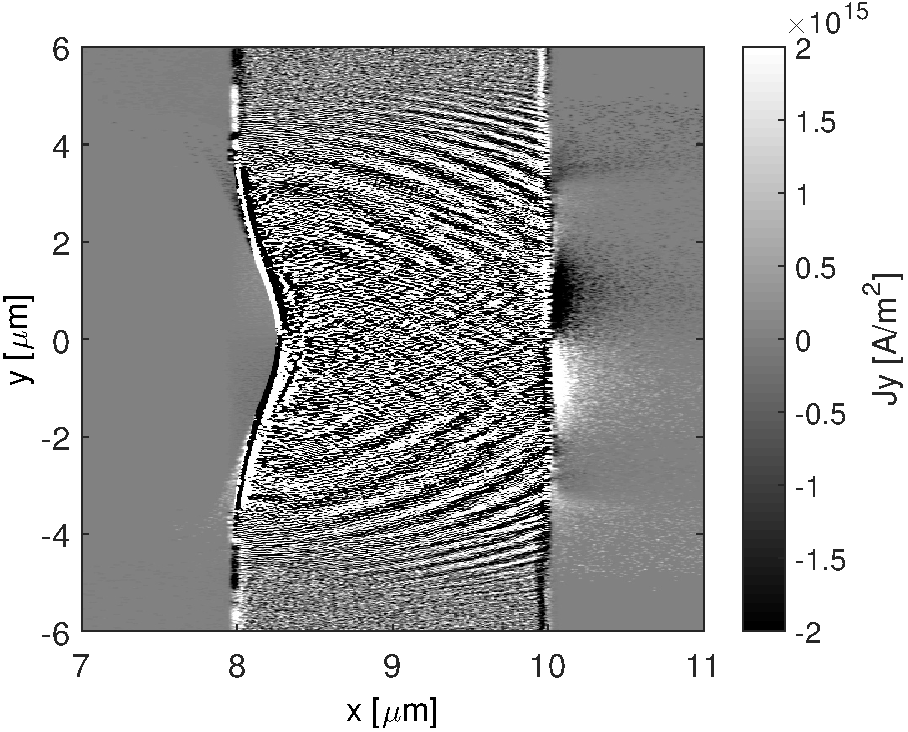
\includegraphics[width=0.45\linewidth]{./img/results/i1e21/2/jy.pdf}}}\\[2mm]
	\caption{The y-component of the current density $ J_{y} $ at the time $ t = 100 \ \mathrm{fs} $ for the case of simulations with the laser intensity I = $ 10^{21} $ W/cm$^2$ and with the beam waist \textbf{(a)} $ w_0 = 0.5 \ \mu\mathrm{m} $, \textbf{(b)} $ w_0 = 2.0 \ \mu\mathrm{m} $.}
	\label{fig:18}
\end{figure}

\floatsetup[figure]{style=plain, subcapbesideposition=top}
\begin{figure}[h!]
	\centering
	\sidesubfloat[]{{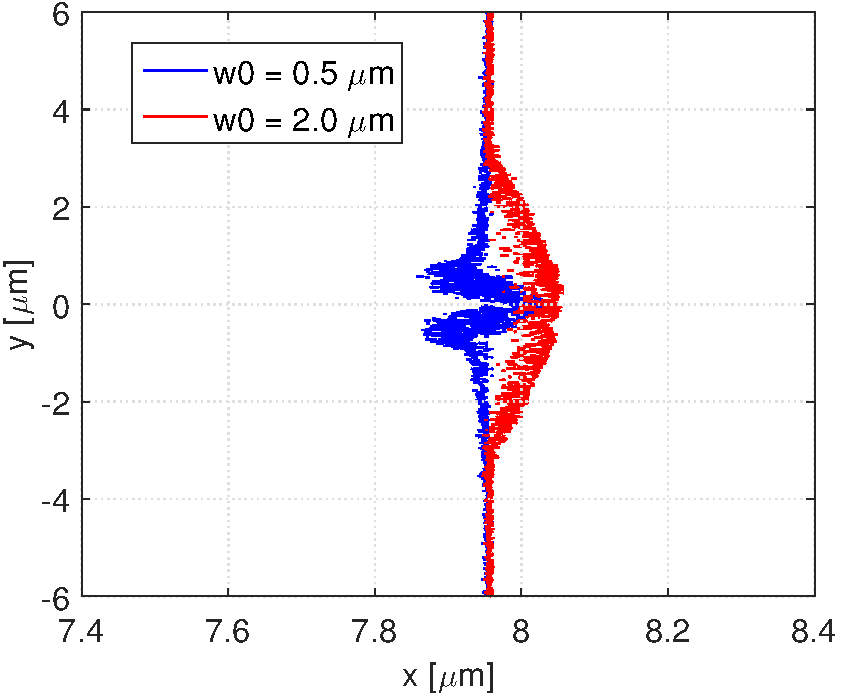
\includegraphics[width=0.445\linewidth]{./img/results/i1e20/dens.pdf}}}
	\hspace{1mm}
	\sidesubfloat[]{{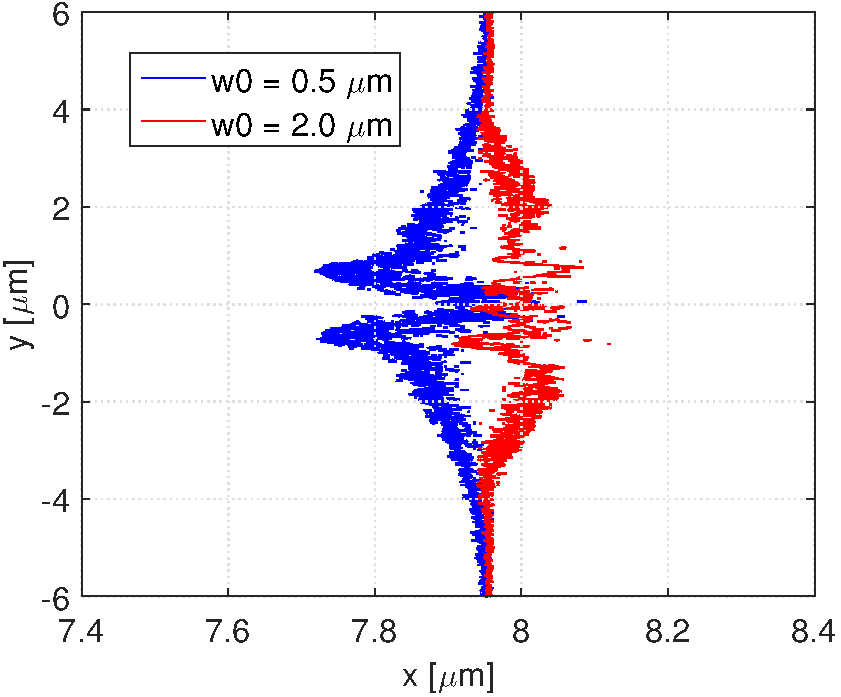
\includegraphics[width=0.445\linewidth]{./img/results/i1e21/dens.pdf}}}
	\caption{Contours of ion critical density for several different beam waists at the time $ t = 100 \ \mathrm{fs} $ for the case of simulations with the laser intensity \textbf{(a)} I = $ 10^{20} $ W/cm$^2$ and \textbf{(b)} I = $ 10^{21} $ W/cm$^2$.}
	\label{fig:15}
\end{figure}

\floatsetup[figure]{style=plain, subcapbesideposition=top}
\begin{figure}[h!]
	\centering
	\sidesubfloat[]{{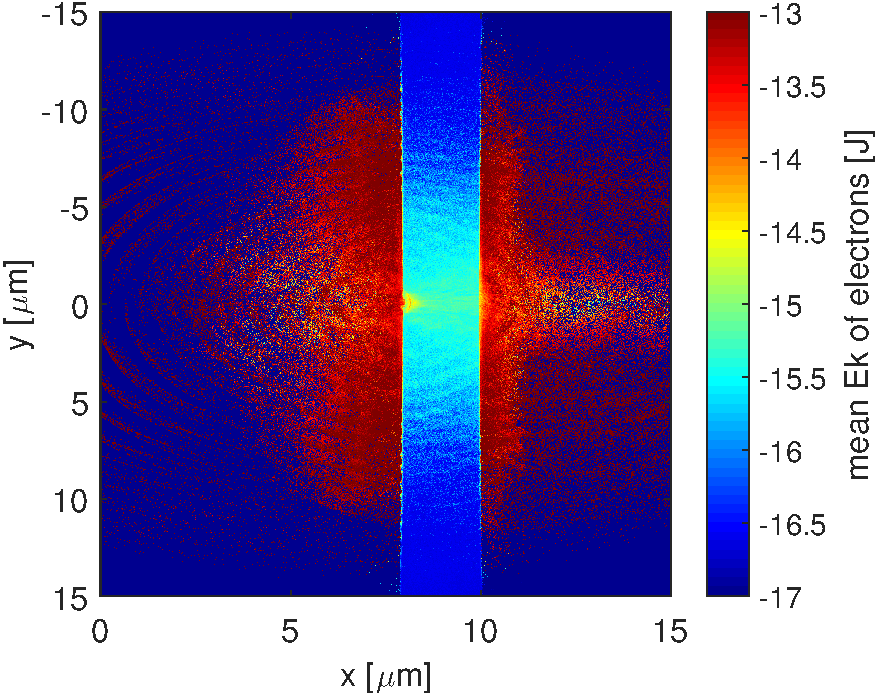
\includegraphics[width=0.45\linewidth]{./img/results/i1e20/05/ekbar.pdf}}}
	\sidesubfloat[]{{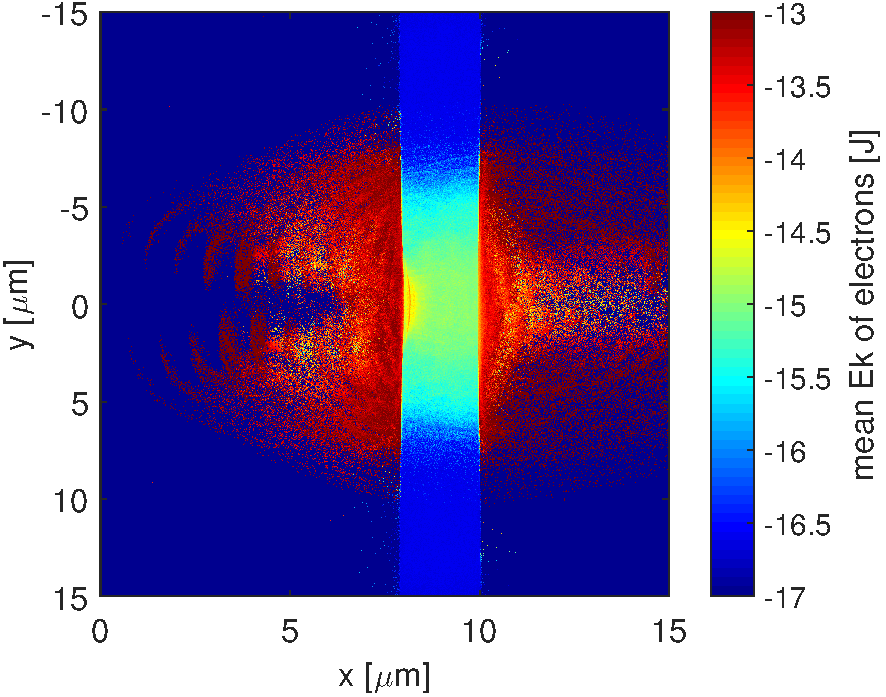
\includegraphics[width=0.45\linewidth]{./img/results/i1e20/2/ekbar.pdf}}}\\[2mm]
	\sidesubfloat[]{{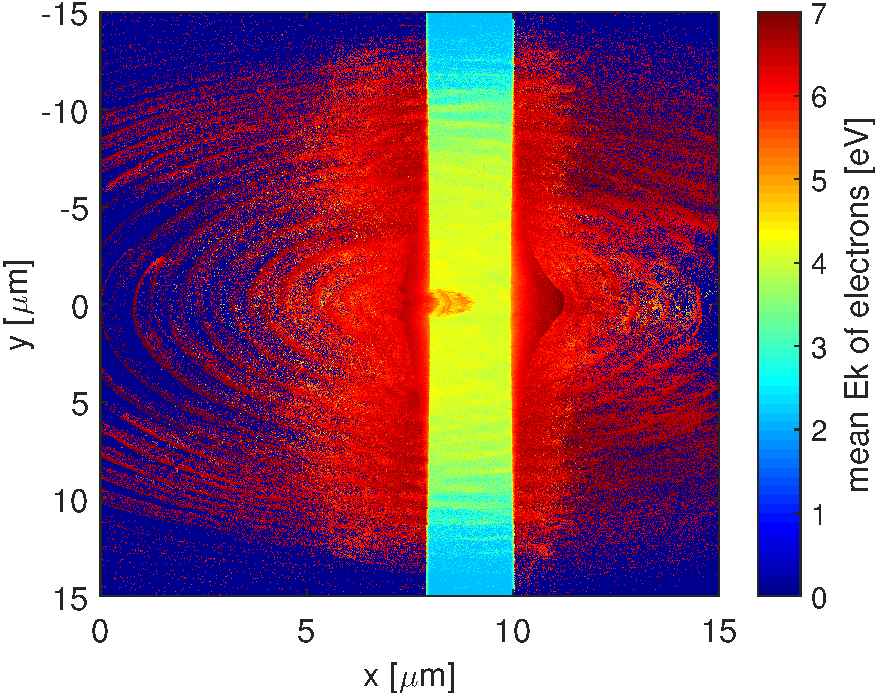
\includegraphics[width=0.45\linewidth]{./img/results/i1e21/05/ekbar.pdf}}}
	\sidesubfloat[]{{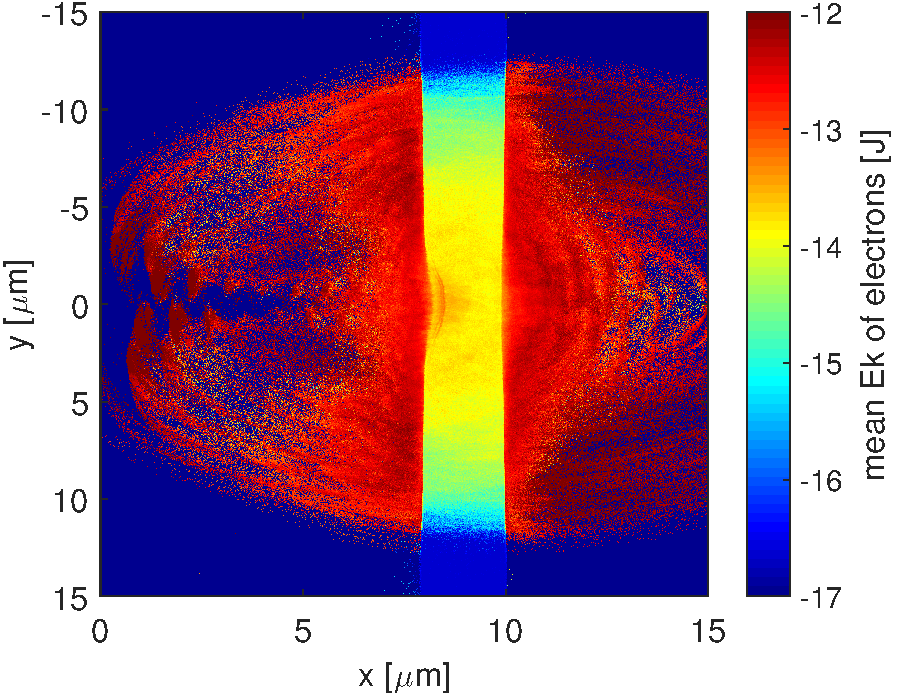
\includegraphics[width=0.45\linewidth]{./img/results/i1e21/2/ekbar.pdf}}}
	\caption{Mean kinetic energy of electrons at the time $ t = 120 \ \mathrm{fs} $ for the case of simulations with the laser intensity I = $ 10^{20} $ W/cm$^2$ and with the beam waist \textbf{(a)} $ w_0 = 0.5 \ \mu\mathrm{m} $, \textbf{(b)} $ w_0 = 2.0 \ \mu\mathrm{m} $ and for the case of simulations with the laser intensity I = $ 10^{21} $ W/cm$^2$ and with the beam waist \textbf{(c)} $ w_0 = 0.5 \ \mu\mathrm{m} $, \textbf{(d)} $ w_0 = 2.0 \ \mu\mathrm{m} $. The colorbars are in logarithmic scale.}
	\label{fig:16}
\end{figure}

\floatsetup[figure]{style=plain, subcapbesideposition=top}
\begin{figure}[h!]
	\centering
	\sidesubfloat[]{{\includegraphics[width=0.45\linewidth]{./img/results/i1e20/05/abs_ex.pdf}}}
	\sidesubfloat[]{{\includegraphics[width=0.45\linewidth]{./img/results/i1e20/2/abs_ex.pdf}}}\\[2mm]
	\sidesubfloat[]{{\includegraphics[width=0.45\linewidth]{./img/results/i1e21/05/abs_ex.pdf}}}
	\sidesubfloat[]{{\includegraphics[width=0.45\linewidth]{./img/results/i1e21/2/abs_ex.pdf}}}
	\caption{Longitudinal electric field ($ E_{x} $) at the time  $ t = 120 \ \mathrm{fs} $ for the case of simulations with the laser intensity I = $ 10^{20} $ W/cm$^2$ and with the beam waist \textbf{(a)} $ w_0 = 0.5 \ \mu\mathrm{m} $, \textbf{(b)} $ w_0 = 2.0 \ \mu\mathrm{m} $ and for the case of simulations with the laser intensity I = $ 10^{21} $ W/cm$^2$ and with the beam waist \textbf{(c)} $ w_0 = 0.5 \ \mu\mathrm{m} $, \textbf{(d)} $ w_0 = 2.0 \ \mu\mathrm{m} $.}
	\label{fig:20}
\end{figure}

\floatsetup[figure]{style=plain, subcapbesideposition=top}
\begin{figure}[h!]
	\centering
	\sidesubfloat[]{{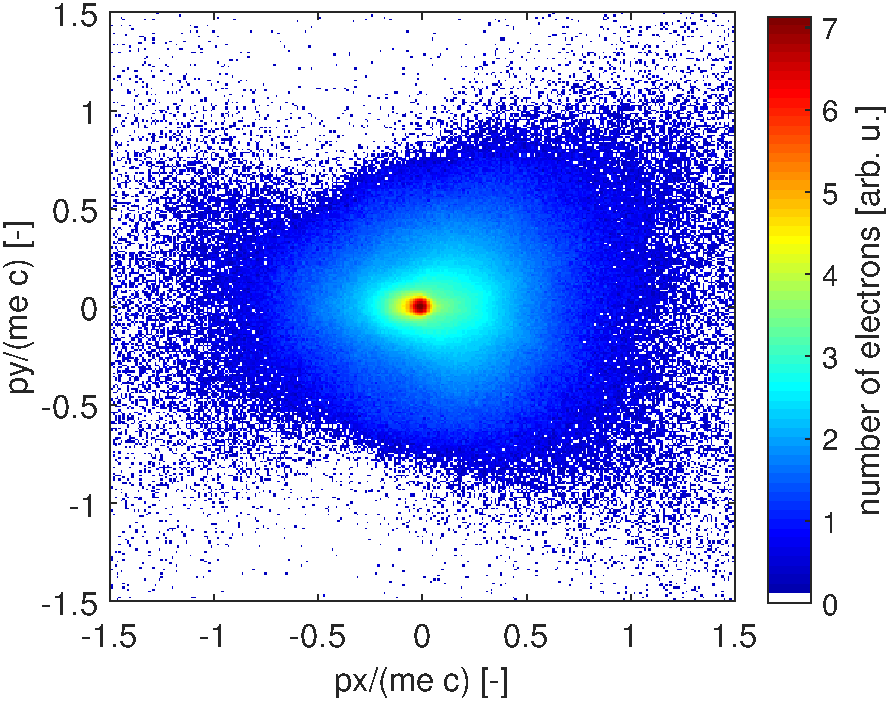
\includegraphics[width=0.45\linewidth]{./img/results/i1e20/05/px_py.pdf}}}
	\sidesubfloat[]{{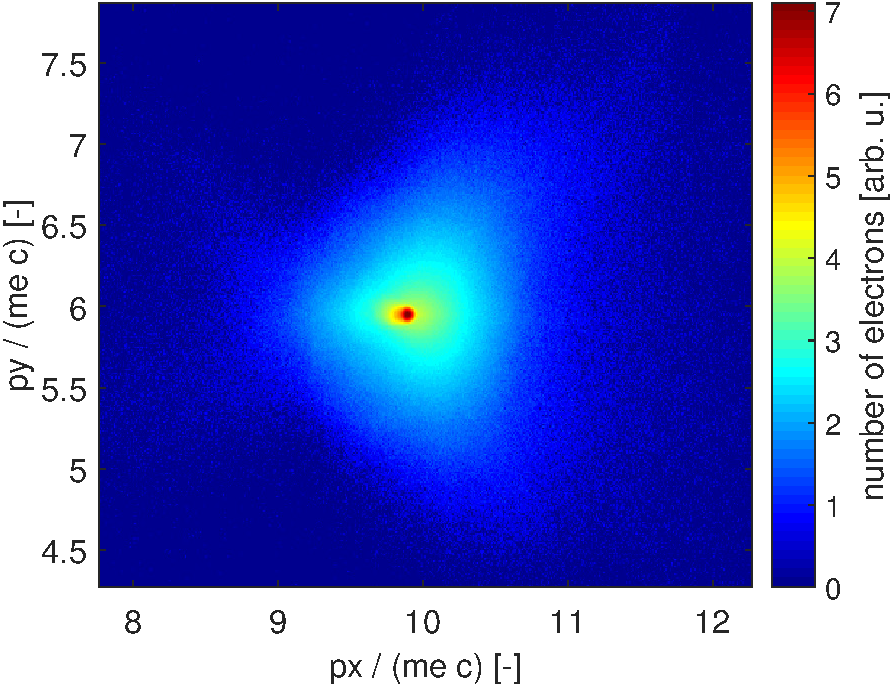
\includegraphics[width=0.45\linewidth]{./img/results/i1e20/2/px_py.pdf}}}\\
	\sidesubfloat[]{{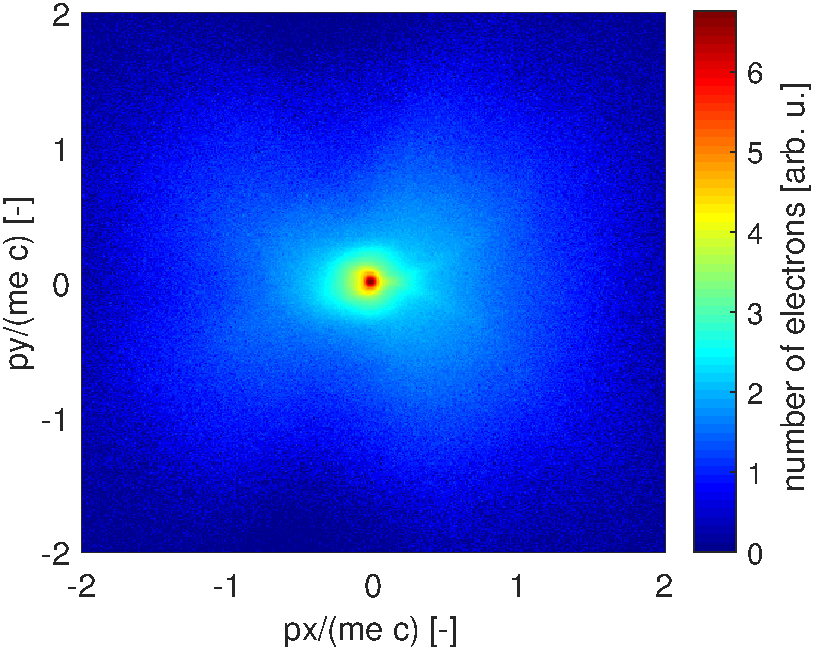
\includegraphics[width=0.45\linewidth]{./img/results/i1e21/05/px_py.pdf}}}
	\sidesubfloat[]{{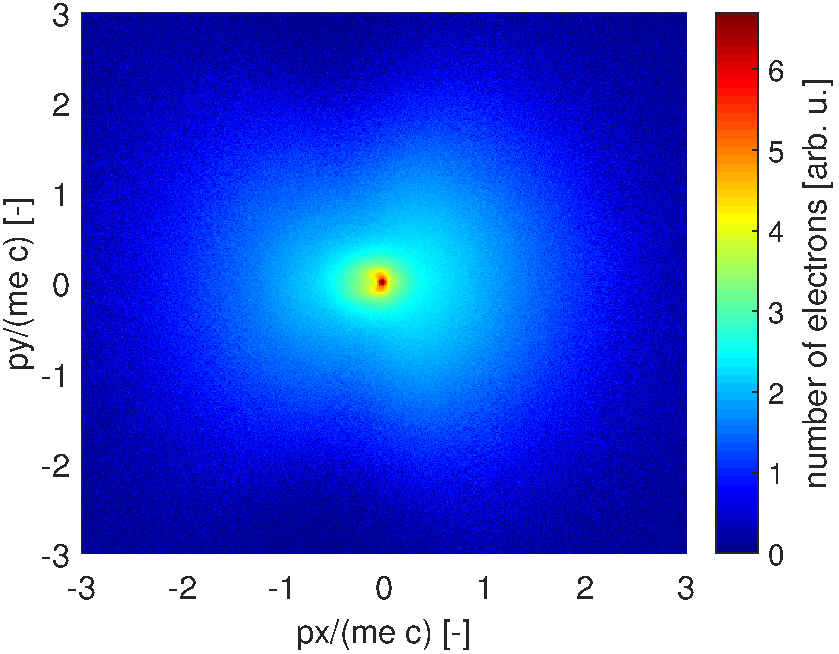
\includegraphics[width=0.45\linewidth]{./img/results/i1e21/2/px_py.pdf}}}
	\caption{Dependency of the x-component of the momentum of electrons on the y-component of the  momentum of electrons at the time $ t = 100 \ \mathrm{fs} $ for the case of simulations with the laser intensity I = $ 10^{20} $ W/cm$^2$ and with the beam waist \textbf{(a)} $ w_0 = 0.5 \ \mu\mathrm{m} $, \textbf{(b)} $ w_0 = 2.0 \ \mu\mathrm{m} $ and for the case of simulations with the laser intensity I = $ 10^{21} $ W/cm$^2$ and with the beam waist \textbf{(c)} $ w_0 = 0.5 \ \mu\mathrm{m} $, \textbf{(d)} $ w_0 = 2.0 \ \mu\mathrm{m} $. The colorbars are in logarithmic scale.}
	\label{fig:12}
\end{figure}

\floatsetup[figure]{style=plain, subcapbesideposition=top}
\begin{figure}[h!]
	\centering
	\sidesubfloat[]{{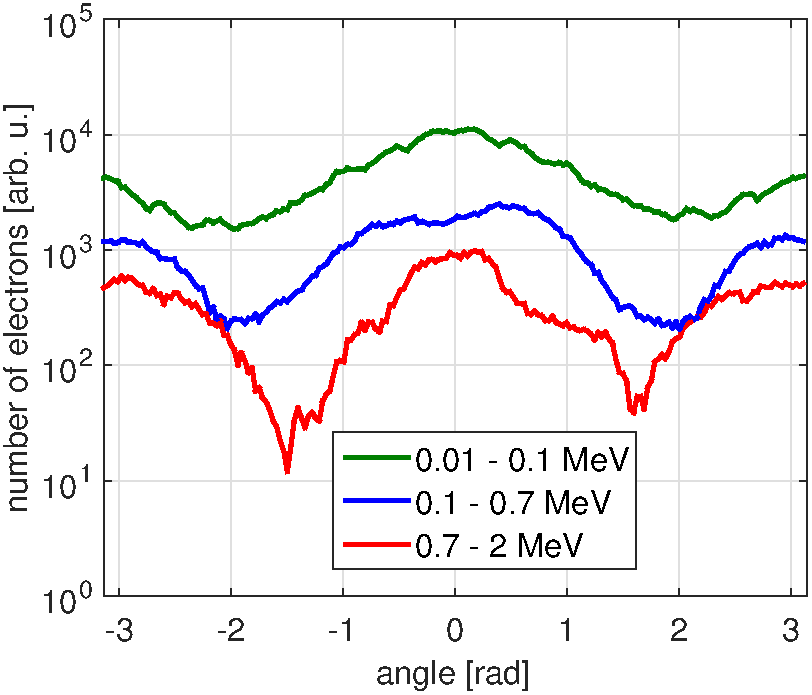
\includegraphics[width=0.445\linewidth]{./img/results/i1e20/05/angles.pdf}}}
	\hspace{1mm}
	\sidesubfloat[]{{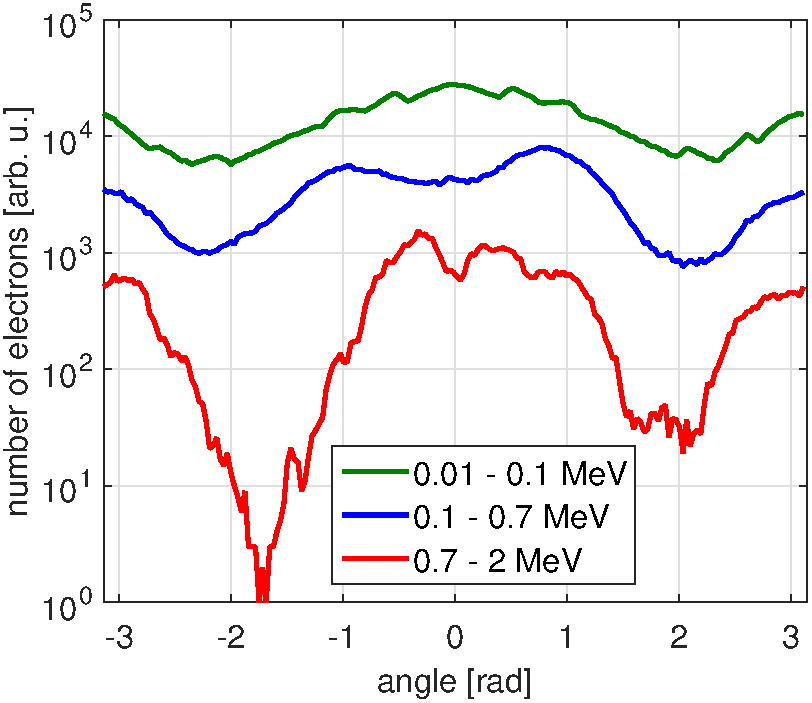
\includegraphics[width=0.445\linewidth]{./img/results/i1e20/2/angles.pdf}}}\\
	\sidesubfloat[]{{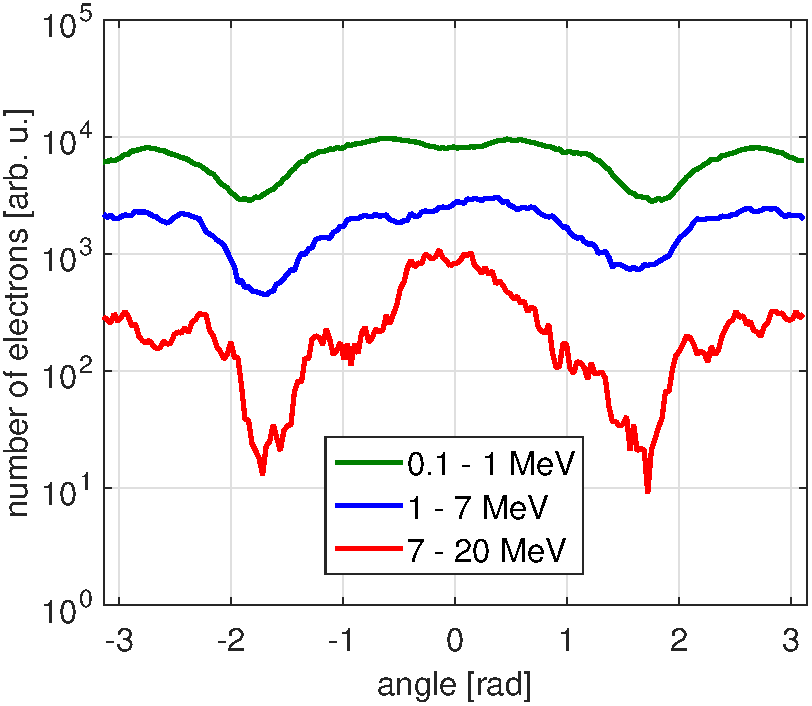
\includegraphics[width=0.445\linewidth]{./img/results/i1e21/05/angles.pdf}}}
	\hspace{1mm}
	\sidesubfloat[]{{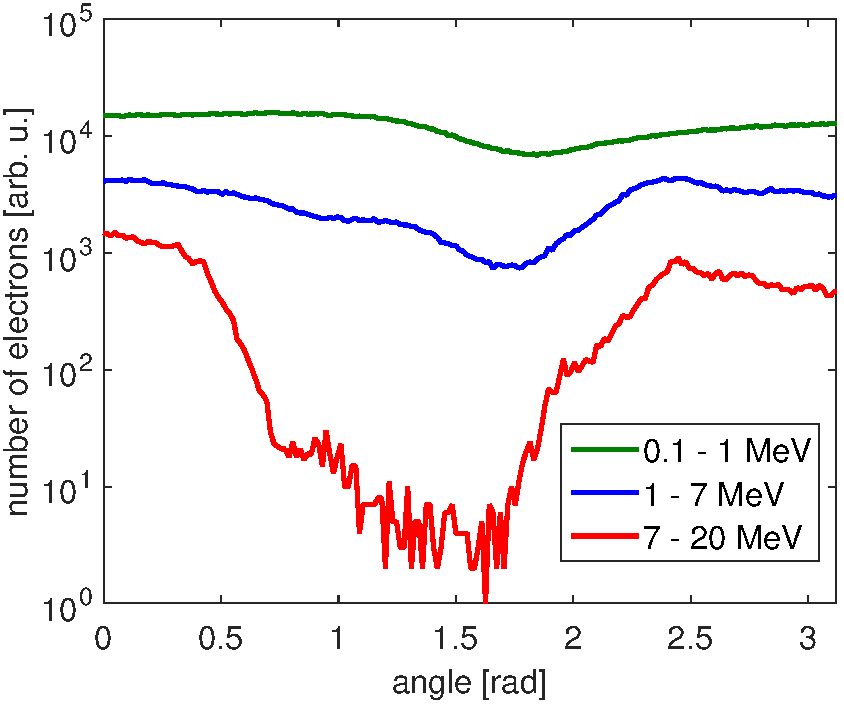
\includegraphics[width=0.445\linewidth]{./img/results/i1e21/2/angles.pdf}}}
	\caption{Distribution of angles determining the direction of movement of electrons (the angle 0 stands for the motion forward) at the time $ t = 100 \ \mathrm{fs} $ for the case of simulations with the laser intensity I = $ 10^{20} $ W/cm$^2$ and with the beam waist \textbf{(a)} $ w_0 = 0.5 \ \mu\mathrm{m} $, \textbf{(b)} $ w_0 = 2.0 \ \mu\mathrm{m} $ and for the case of simulations with the laser intensity I = $ 10^{21} $ W/cm$^2$ and with the beam waist \textbf{(c)} $ w_0 = 0.5 \ \mu\mathrm{m} $, \textbf{(d)} $ w_0 = 2.0 \ \mu\mathrm{m} $. Electrons are divided into three energetic intervals.}
	\label{fig:13}
\end{figure}

\floatsetup[figure]{style=plain, subcapbesideposition=top}
\begin{figure}[h!]
	\centering
	\sidesubfloat[]{{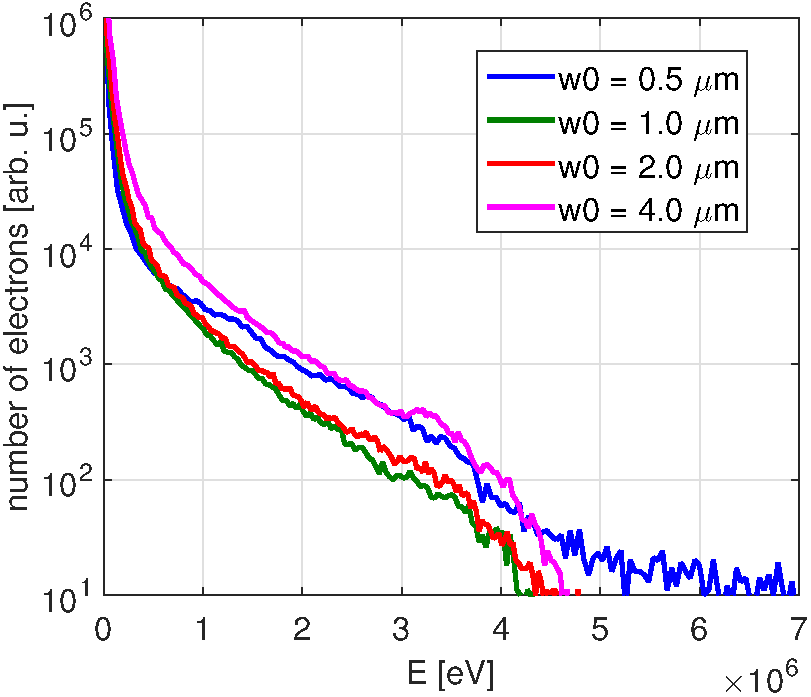
\includegraphics[width=0.445\linewidth]{./img/results/i1e20/dist_e.pdf}}}
	\hspace{1mm}
	\sidesubfloat[]{{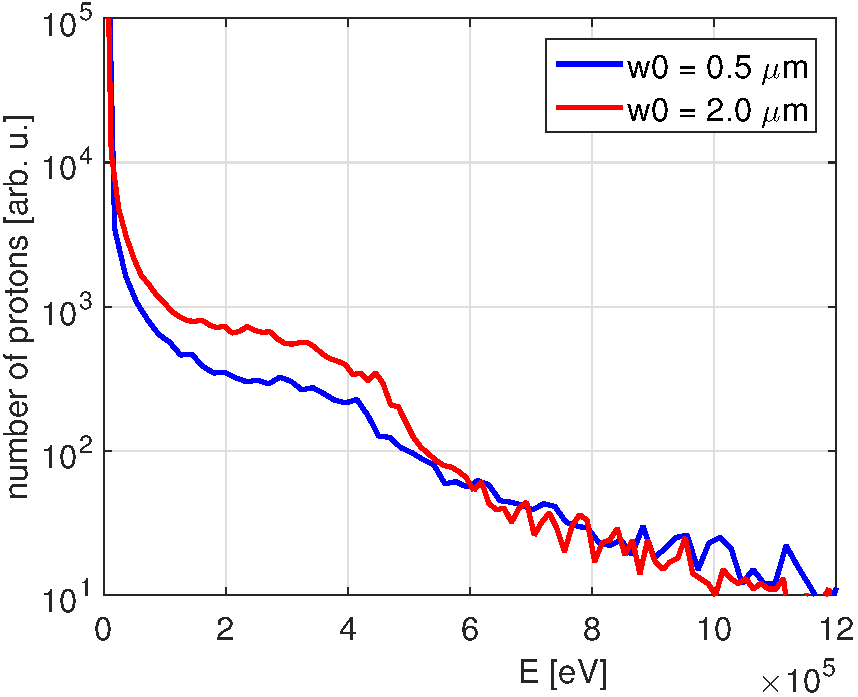
\includegraphics[width=0.445\linewidth]{./img/results/i1e20/dist_p.pdf}}}\\[2mm]
	\sidesubfloat[]{{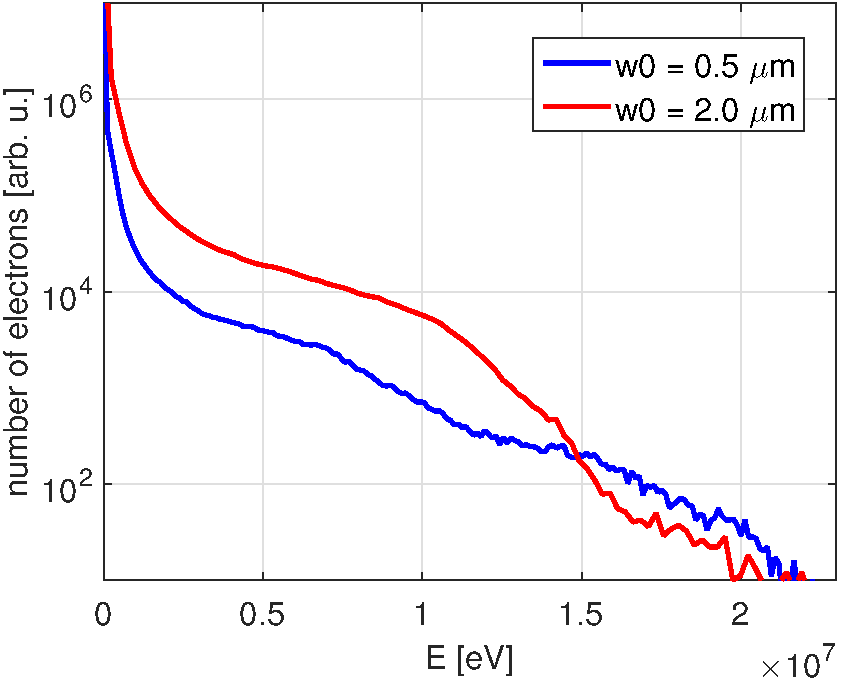
\includegraphics[width=0.445\linewidth]{./img/results/i1e21/dist_e.pdf}}}
	\hspace{1mm}
	\sidesubfloat[]{{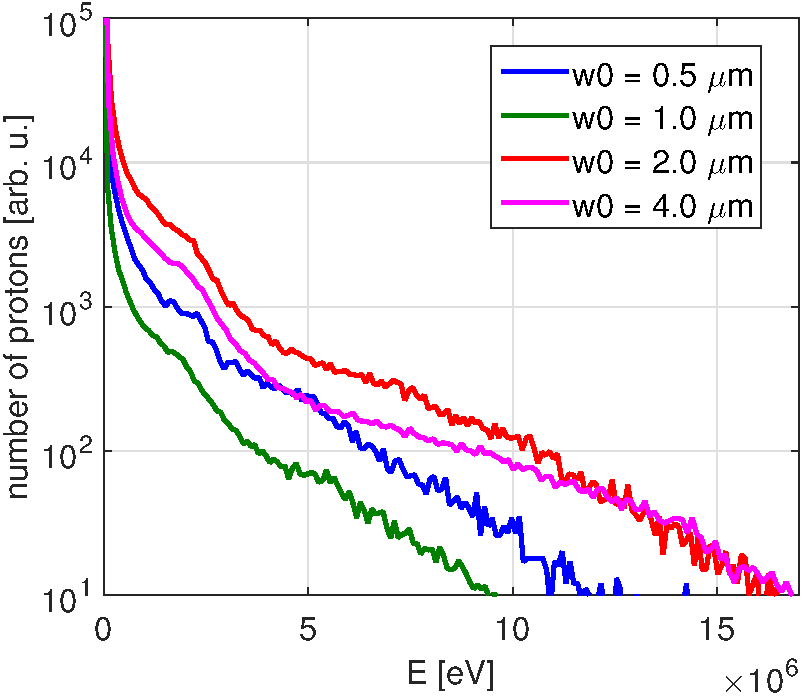
\includegraphics[width=0.445\linewidth]{./img/results/i1e21/dist_p.pdf}}}
	\caption{Energy distribution functions of electrons for several different beam waists at the time $ t = 100 \ \mathrm{fs} $ for the case of simulations with the laser intensity \textbf{(a)} I = $ 10^{20} $ W/cm$^2$ and \textbf{(c)} I = $ 10^{21} $ W/cm$^2$. Energy distribution functions of ions for several different beam waists at the time $ t = 150 \ \mathrm{fs} $ for the case of simulations with the laser intensity \textbf{(b)} I = $ 10^{20} $ W/cm$^2$ and \textbf{(d)} I = $ 10^{21} $ W/cm$^2$.}
	\label{fig:14}
\end{figure}